\chapter{Calcualtion results and analysis}
Once all the experiment data and parameters are determined, the results 
of the calculation should be presented and analyzed. Thus, the 
accuracy, consistency, pros and cons of the virtual experiment 
platform and temperature estimation algorithm can be systematically 
analyzed.

\section{Calculation results}
In virtual experiment platform and temperature estimation algorithms, emissivity is considered as a 
function of radiation wavelength and temperature. Consequently, it varies with changes in 
temperature and radiation wavelength. This variability is advantageous for enhancing algorithm 
precision but introduces difficulties in visualizing computation results. Furthermore, 
temperature estimation algorithm doesn't directly calculate the emissivity of materials; 
instead, the algorithm optimize the parameters $k$ of the emissivity model. 
Thus, the emissivity data of each point is a function of wavelength $\lambda$ and thus
cannot be directly visualized. To address this, a simplified 
approach for visualizing emissivity is introduced, which allows for a more intuitive 
representation of emissivity without compromising the accuracy of the computational process.

\begin{equation}
    \label{eq: emi_average}
    \varepsilon_{sim} = \overline{\varepsilon(\lambda)} 
\end{equation}

Eq.\ref{eq: emi_average} presents the mathematical expression for this simplification. 
$\varepsilon_{sim}$ represents the simplified emissivity value, and $\varepsilon(\lambda)$ denotes 
the emissivity model's value at wavelength $\lambda$. In other words, in this work, the 
visualization of emissivity is derived from the average value of emissivity model data 
within the wavelength range of 500 to 1000 nanometers.


By employing the same simplification method in the generation of experimental data and 
subsequent temperature estimation algorithm, the validity of the program's verification is 
ensured. This consistency guarantees that the comparison between the data used for 
validation remains effective and reliable throughout the process.


After obtaining a standardized emissivity visualization method, it is necessary to validate the 
calculation results. For the convenience of validation, several data that cannot be 
obtained in real experiments, such as temperature and emissivity of hypothetical material 
have been saved in several files in the virtual experiment platform and used to 
check the accuracy in validation process.


\subsection{Raw experiment data from virtual experiment platform}
In order to assess the performance of the temperature estimation algorithm 
at different temperatures and facilitate visual analysis, a linear temperature 
distribution is employed during the validation process. The background 
temperature is set to 1000K, while the center point's temperature is 
set at 1900K. Details is shown in Fig.\ref{fig: t_field}. Simultaneously, the melting point of the hypothetical material 
is defined as 1600K (except black body and gray body hypothetical material). 
This approach allows for the comparison of data obtained 
from the virtual experimental platform with that from real experiments, 
while checking the accuracy of the temperature estimation algorithm in 
both solid and liquid phase of the hypothetical material.


\begin{figure}[htbp]
    \centering
    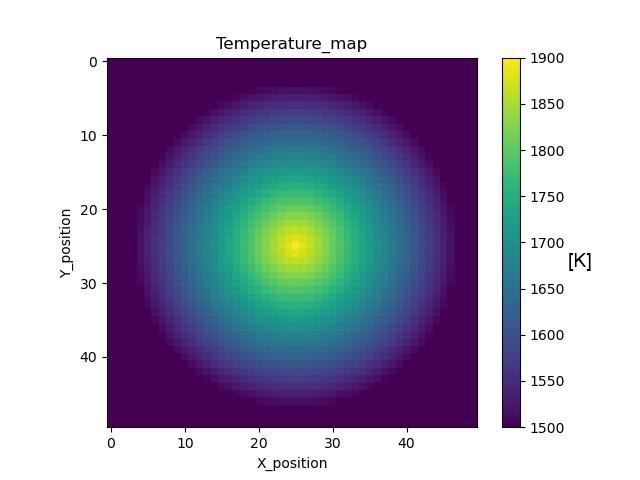
\includegraphics[width=0.8\textwidth]{figures/t_field.jpg}
    \caption{Temperature field used in validation}
    \label{fig: t_field}
\end{figure}


After obtaining a temperature field, the virtual experimental platform 
used the aforementioned 12 different emissivity models to generate 12 
different sets of experimental data. This approach simulated the radiative 
behavior of 12 hypothetical materials under identical temperature conditions 
in the virtual experiment platform.

\begin{figure}[htbp]
    \centering
    \begin{minipage}{\textwidth}
        \centering
        \begin{subfigure}{0.45\textwidth}
            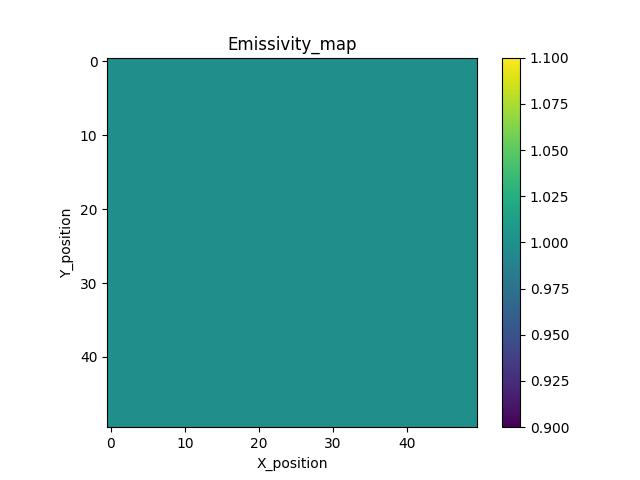
\includegraphics[width=\textwidth]{figures/raw_data/0/emi_field.jpg}
        \end{subfigure}
        \begin{subfigure}{0.45\textwidth}
            \centering
            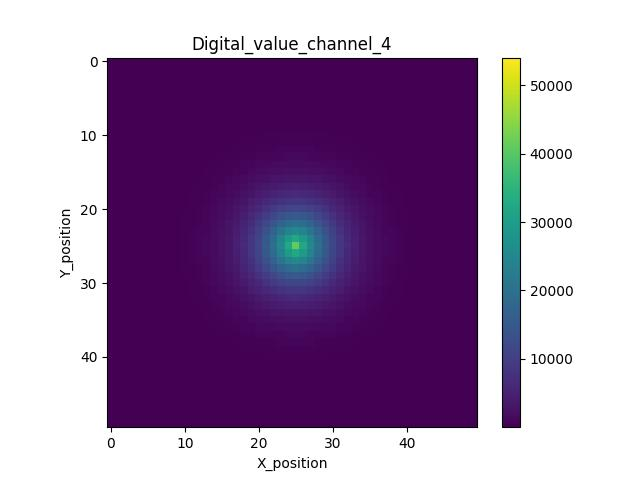
\includegraphics[width=\textwidth]{figures/raw_data/0/digital_value_channel_4.jpg}
        \end{subfigure}
        \subcaption{Black body}
        \label{fig: raw_data_0}
    \end{minipage}\\
    \begin{minipage}{\textwidth}
        \centering
        \begin{subfigure}{0.45\textwidth}
            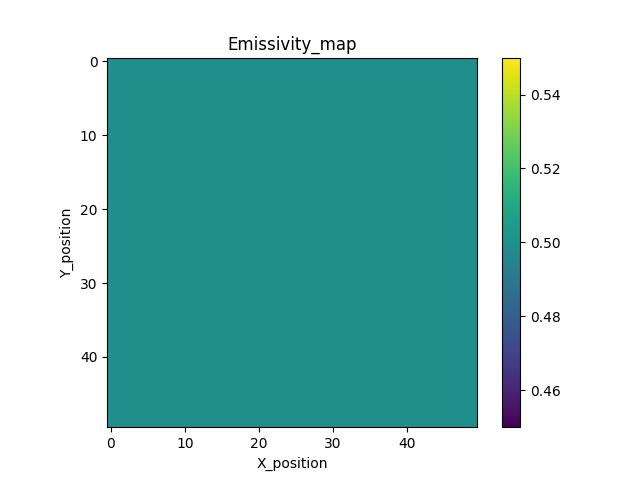
\includegraphics[width=\textwidth]{figures/raw_data/1/emi_field.jpg}
        \end{subfigure}
        \begin{subfigure}{0.45\textwidth}
            \centering
            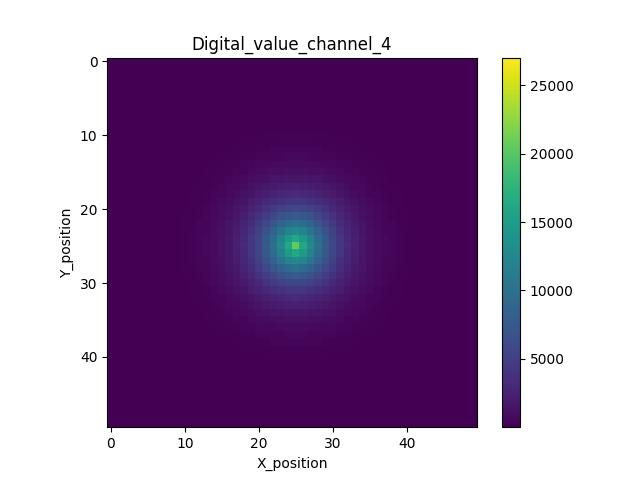
\includegraphics[width=\textwidth]{figures/raw_data/1/digital_value_channel_4.jpg}
        \end{subfigure}
        \subcaption{Gray body}
        \label{fig: raw_data_1}
    \end{minipage}\\
    \begin{minipage}{\textwidth}
        \centering
        \begin{subfigure}{0.45\textwidth}
            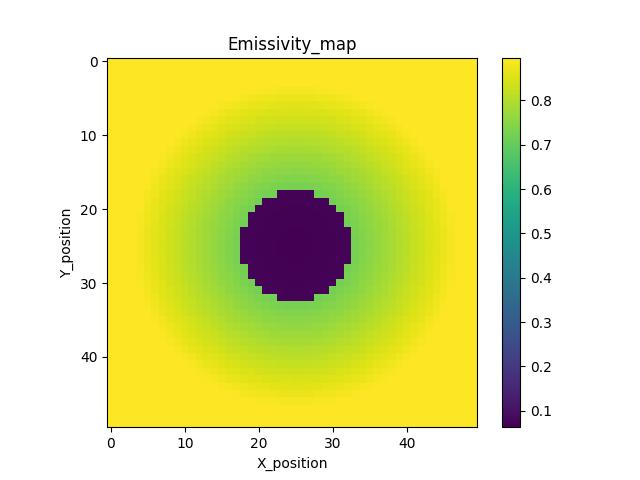
\includegraphics[width=\textwidth]{figures/raw_data/21/emi_field.jpg}
        \end{subfigure}
        \begin{subfigure}{0.45\textwidth}
            \centering
            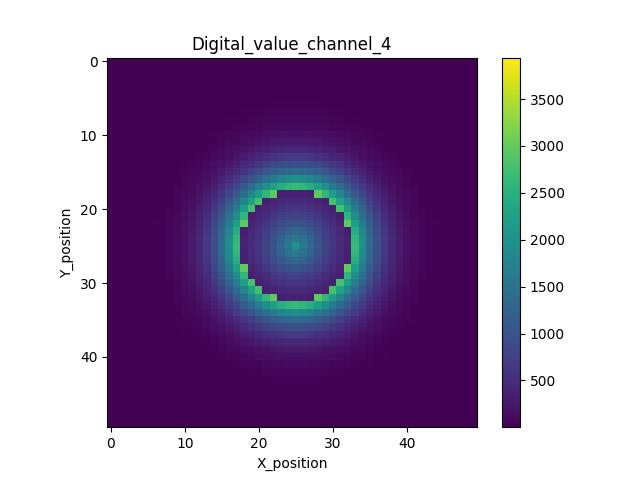
\includegraphics[width=\textwidth]{figures/raw_data/21/digital_value_channel_4.jpg}
        \end{subfigure}
        \subcaption{Model 1}
        \label{fig: raw_data_21}
    \end{minipage}\\
    \begin{minipage}{\textwidth}
        \centering
        \begin{subfigure}{0.45\textwidth}
            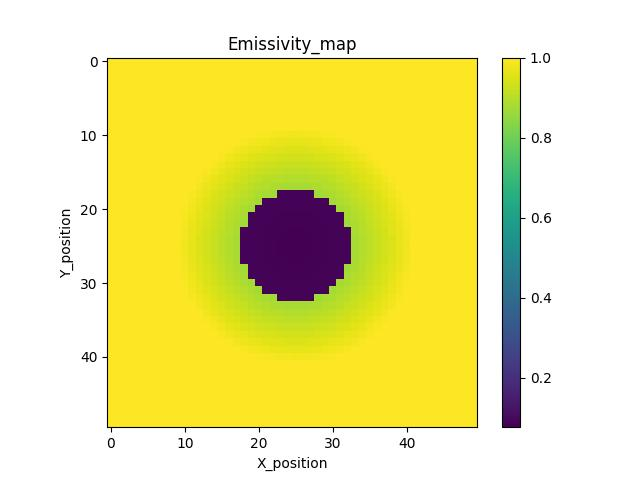
\includegraphics[width=\textwidth]{figures/raw_data/32/emi_field.jpg}
        \end{subfigure}
        \begin{subfigure}{0.45\textwidth}
            \centering
            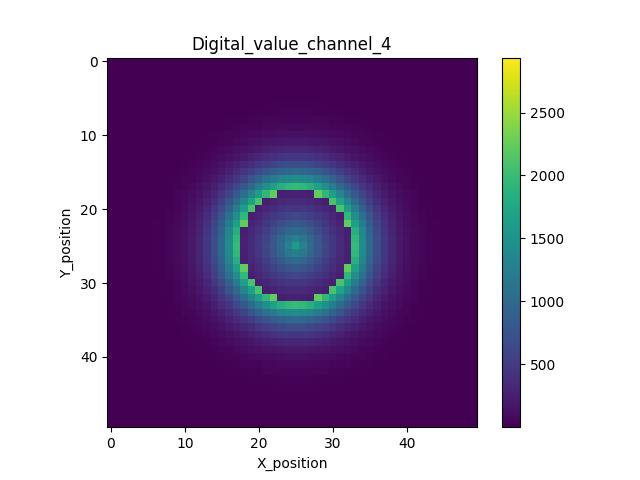
\includegraphics[width=\textwidth]{figures/raw_data/32/digital_value_channel_4.jpg}
        \end{subfigure}
        \subcaption{Model 8}
        \label{fig: raw_data_32}
    \end{minipage}
    \caption{Emissivity field and digital value of radiation intensity in channel 4 for 
    black body material(\subref{fig: raw_data_0}), gray body material(\subref{fig: raw_data_1}), 
    material based on model 1(\subref{fig: raw_data_21}) and model 8(\subref{fig: raw_data_32})}
    \label{fig: raw_data}
\end{figure}

As a result, Fig.\ref{fig: raw_data} displays the emissivity fields generated by defferent
model along with their corresponding radiation intensities. To conserve space, 
digital values of channel 4 in each experiment data were chosen as 
representatives of the intensity data.


It can be observed that in blackbody and gray body materials, emissivity is not 
dependent on the material's temperature or status. As a result, the emissivity 
field exhibits a uniform color distribution. This characteristic also leads to a 
situation in the calculation of radiation intensity, where the physical values 
received by the virtual camera show a maximum at the center point and decrease 
as the temperature decreases.


However, in more general material models, such as Model 1 and Model 8, emissivity 
undergoes a discontinuity when the material transitions from the solid state to 
the liquid state. This is due to the fact that the emissivity of liquid phase 
is smaller than that of solid phase. Consequently, the radiation intensity 
received by the virtual camera decreases at the boundary when the material 
changes from solid to a liquid. Subsequently, at the center point, the radiation 
intensity emitted by the hypothetical material increases again due to the rise in 
temperature. This phenomenon results in a bright halo appearing in the digital 
value of channel 4 in the images. The center of this 
halo exhibits a point with higher brightness level.


Indeed, the non-uniform intensity distribution caused by different emissivity 
characteristics of materials can lead to challenges for the subsequent 
temperature estimation algorithm. The intensity distribution along wavelength 
differs due to the different emissivity model of the hypothetical material. 
Consequently, in the curve fit algorithm, the most suitable emissivity model for 
the current material may change accordingly. Therefore, particular attention 
should be given to the phase transition of the hypothetical material in the 
context of temperature estimation.


After investigating the impact of different emissivity models on material 
radiative characteristics, it is necessary to explore the relationship between 
digital values of radiation intenstiy across different channels. 
Fig.\ref{fig: channel} displays the images of a material based on Model 1 at a 
temperature of 1900K, captured using 8 different channels. In this image, 
it can be observed that the intensity received by the virtual camera increases 
with the channel number.

\begin{figure}[htbp]
    \centering
    \begin{minipage}{0.10\textwidth}
        \centering
        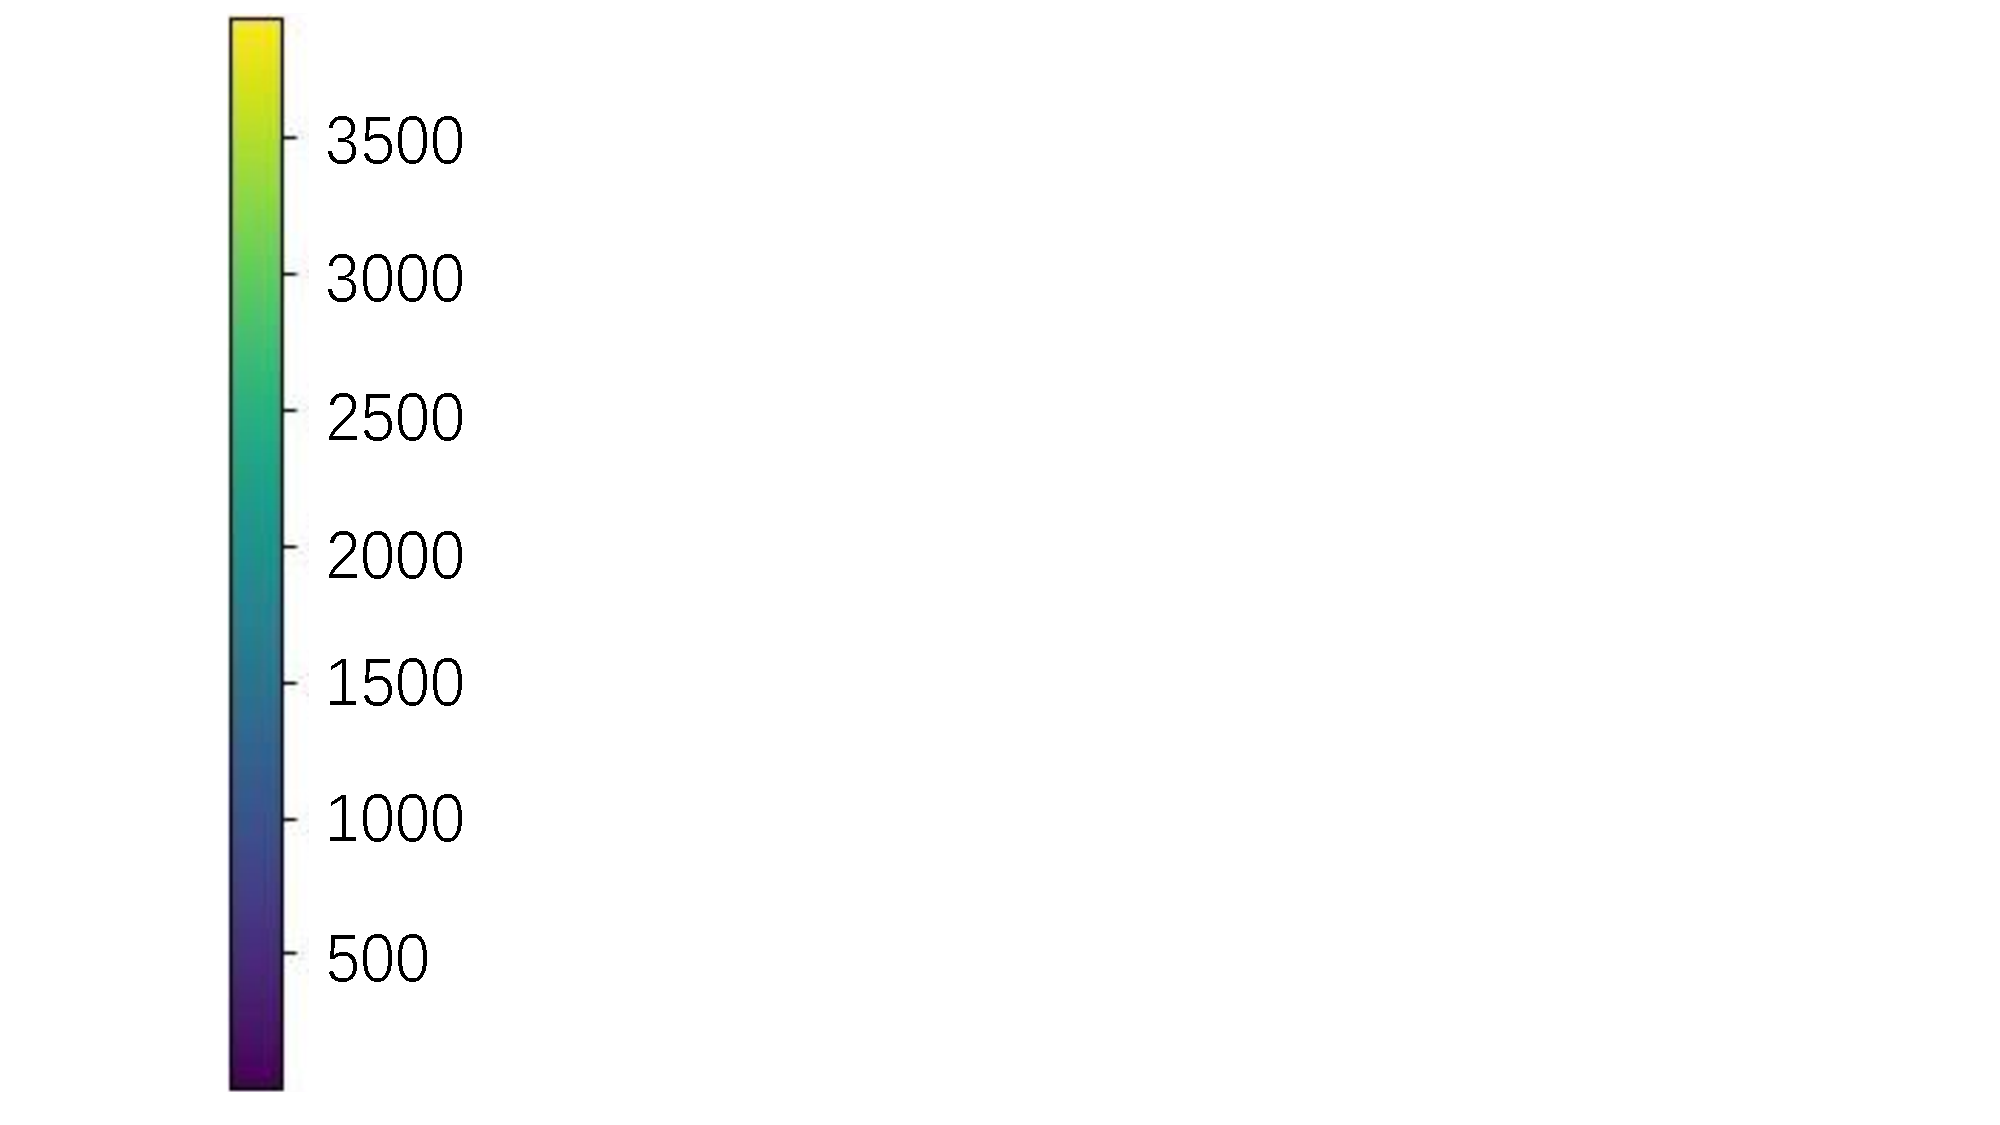
\includegraphics[width=\textwidth]{figures/raw_data/21/color_bar.pdf}
    \end{minipage}
    \begin{minipage}{0.87\textwidth}
        \centering
        \begin{subfigure}{0.23\textwidth}
            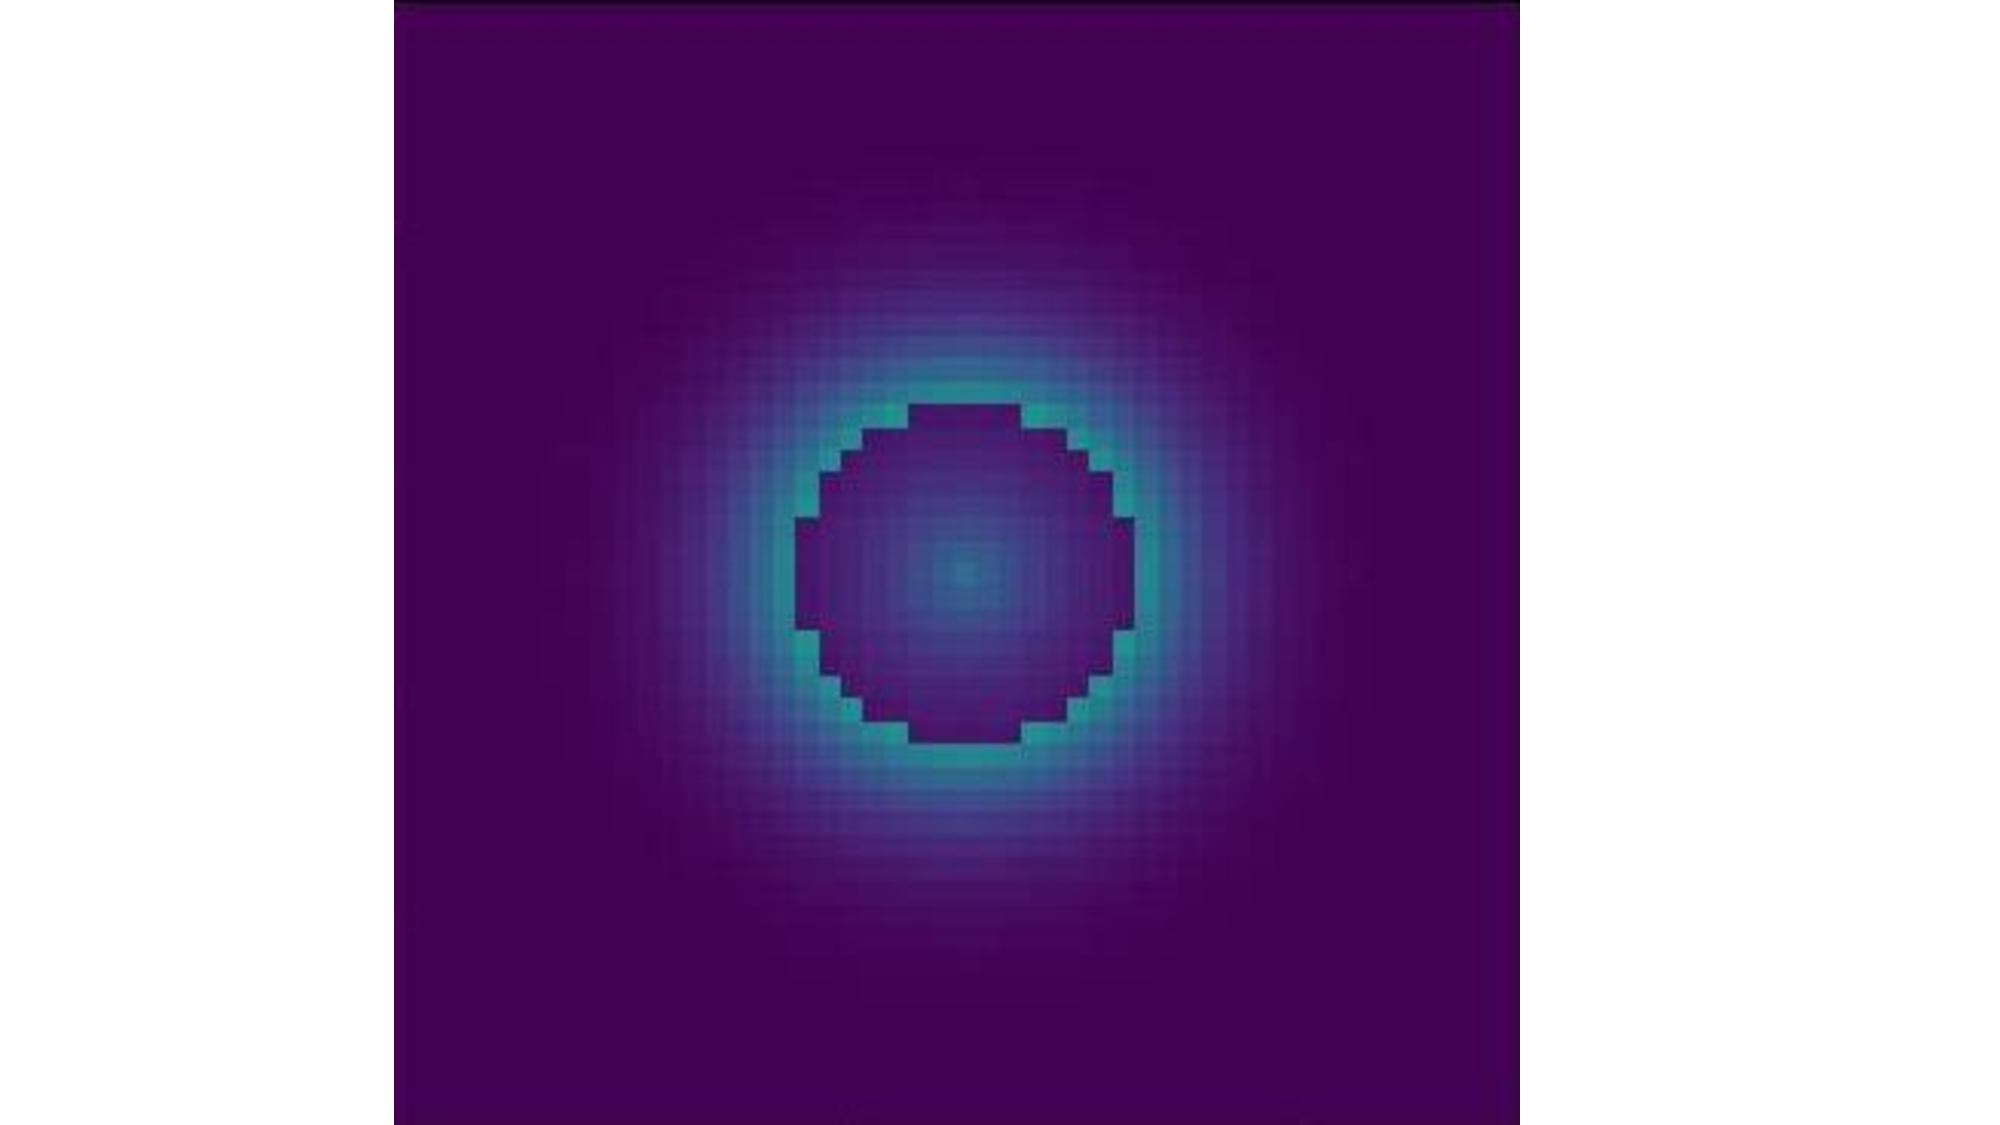
\includegraphics[width=\textwidth]{figures/raw_data/21/channel_1.pdf}
            \caption{Channel 1}
        \end{subfigure}
        \begin{subfigure}{0.23\textwidth}
            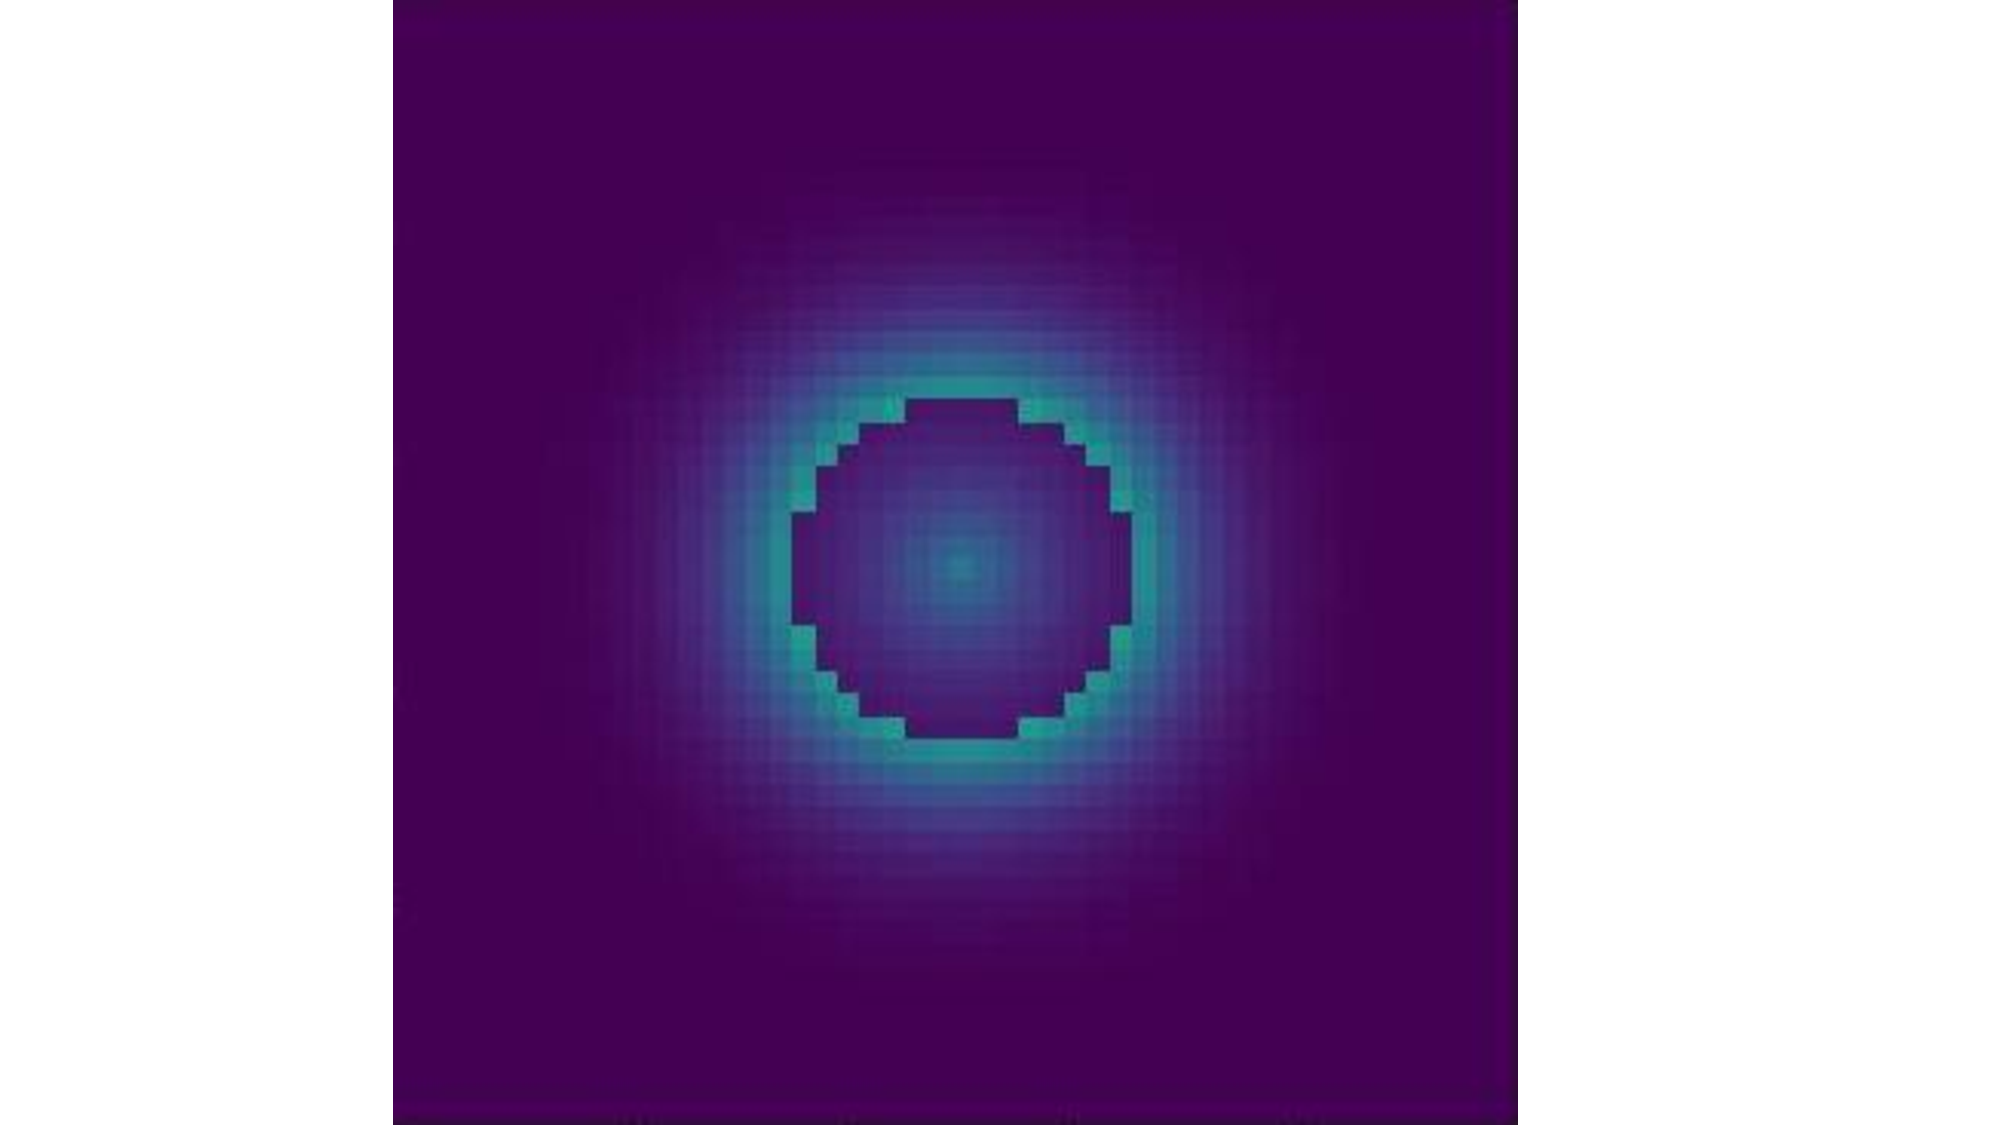
\includegraphics[width=\textwidth]{figures/raw_data/21/channel_2.pdf}
            \caption{Channel 2}
        \end{subfigure}
        \begin{subfigure}{0.23\textwidth}
            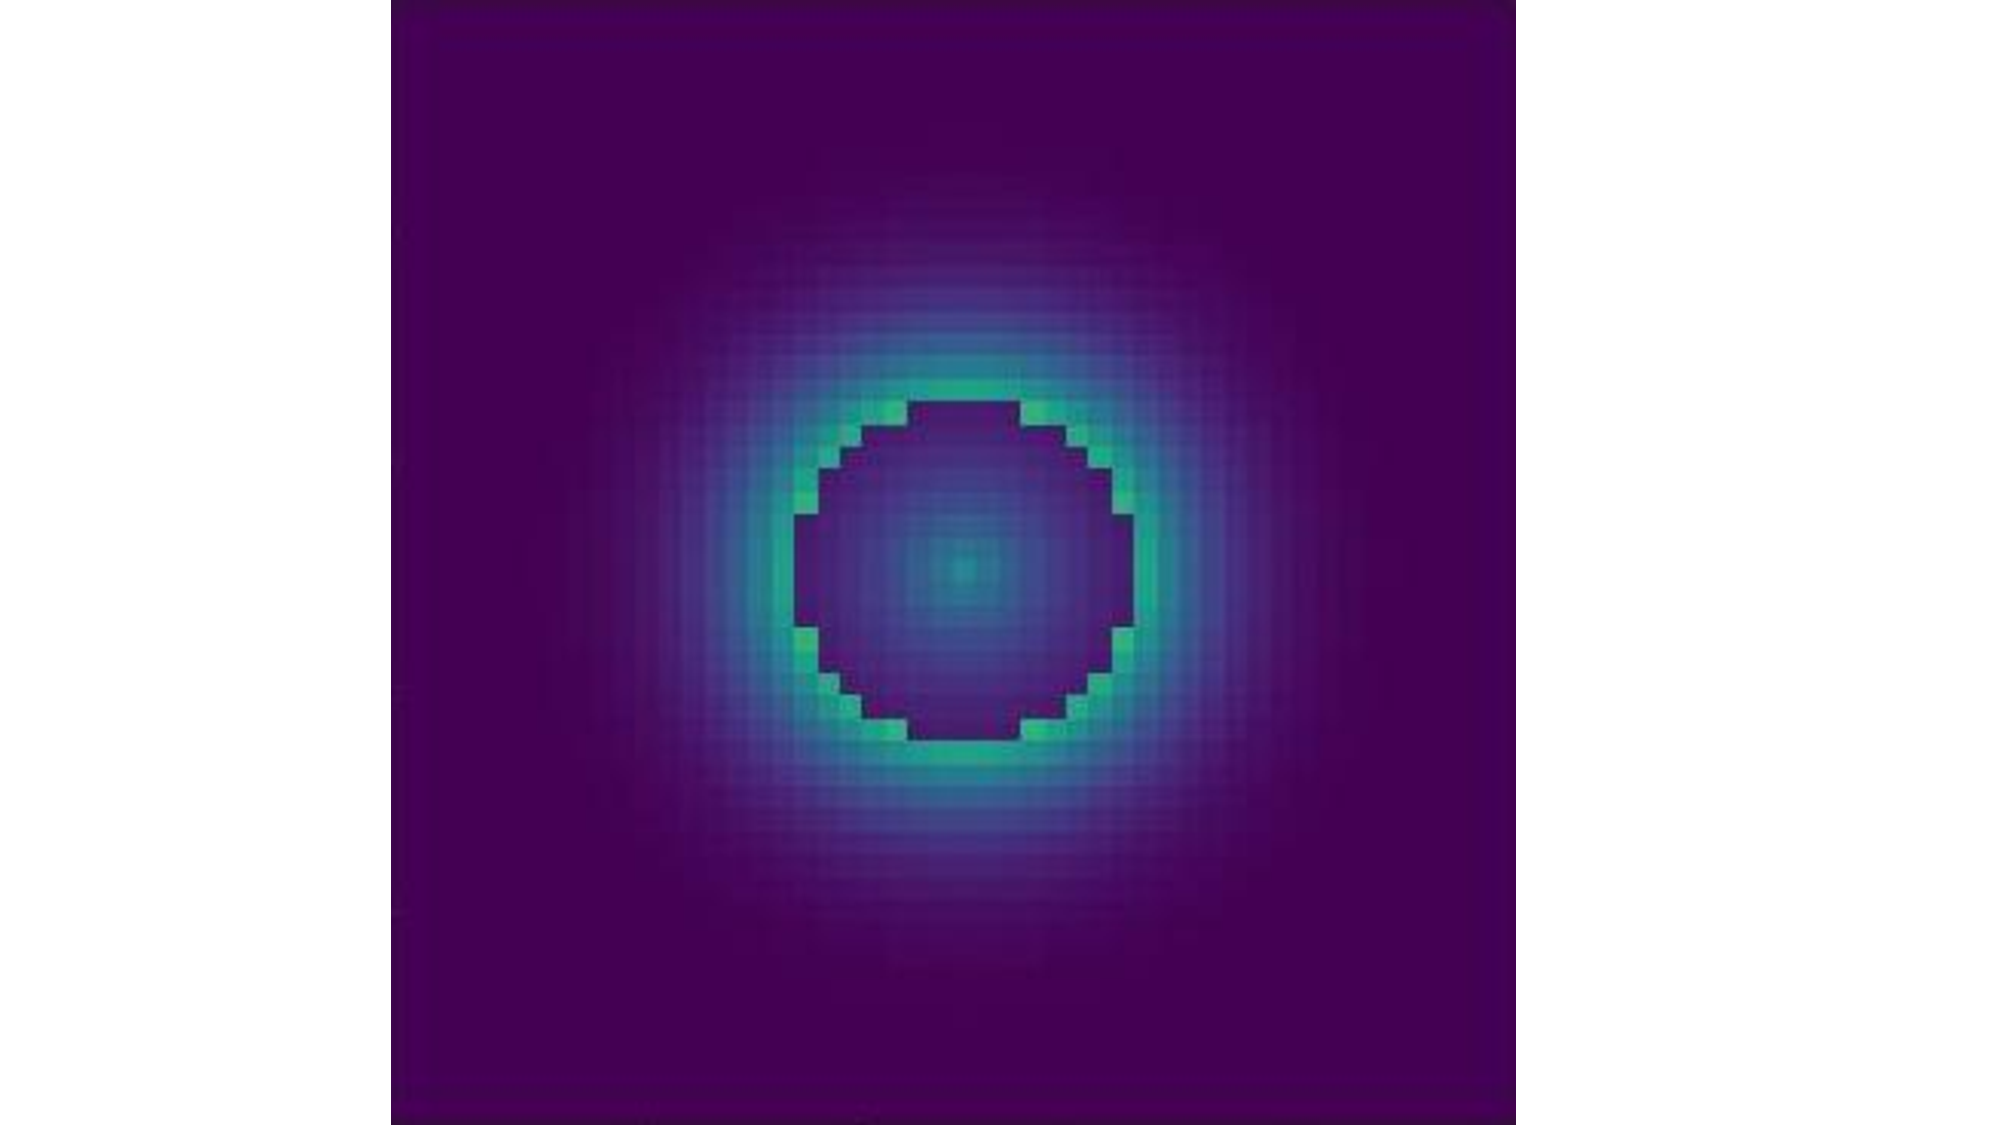
\includegraphics[width=\textwidth]{figures/raw_data/21/channel_3.pdf}
            \caption{Channel 3}
        \end{subfigure}
        \begin{subfigure}{0.23\textwidth}
            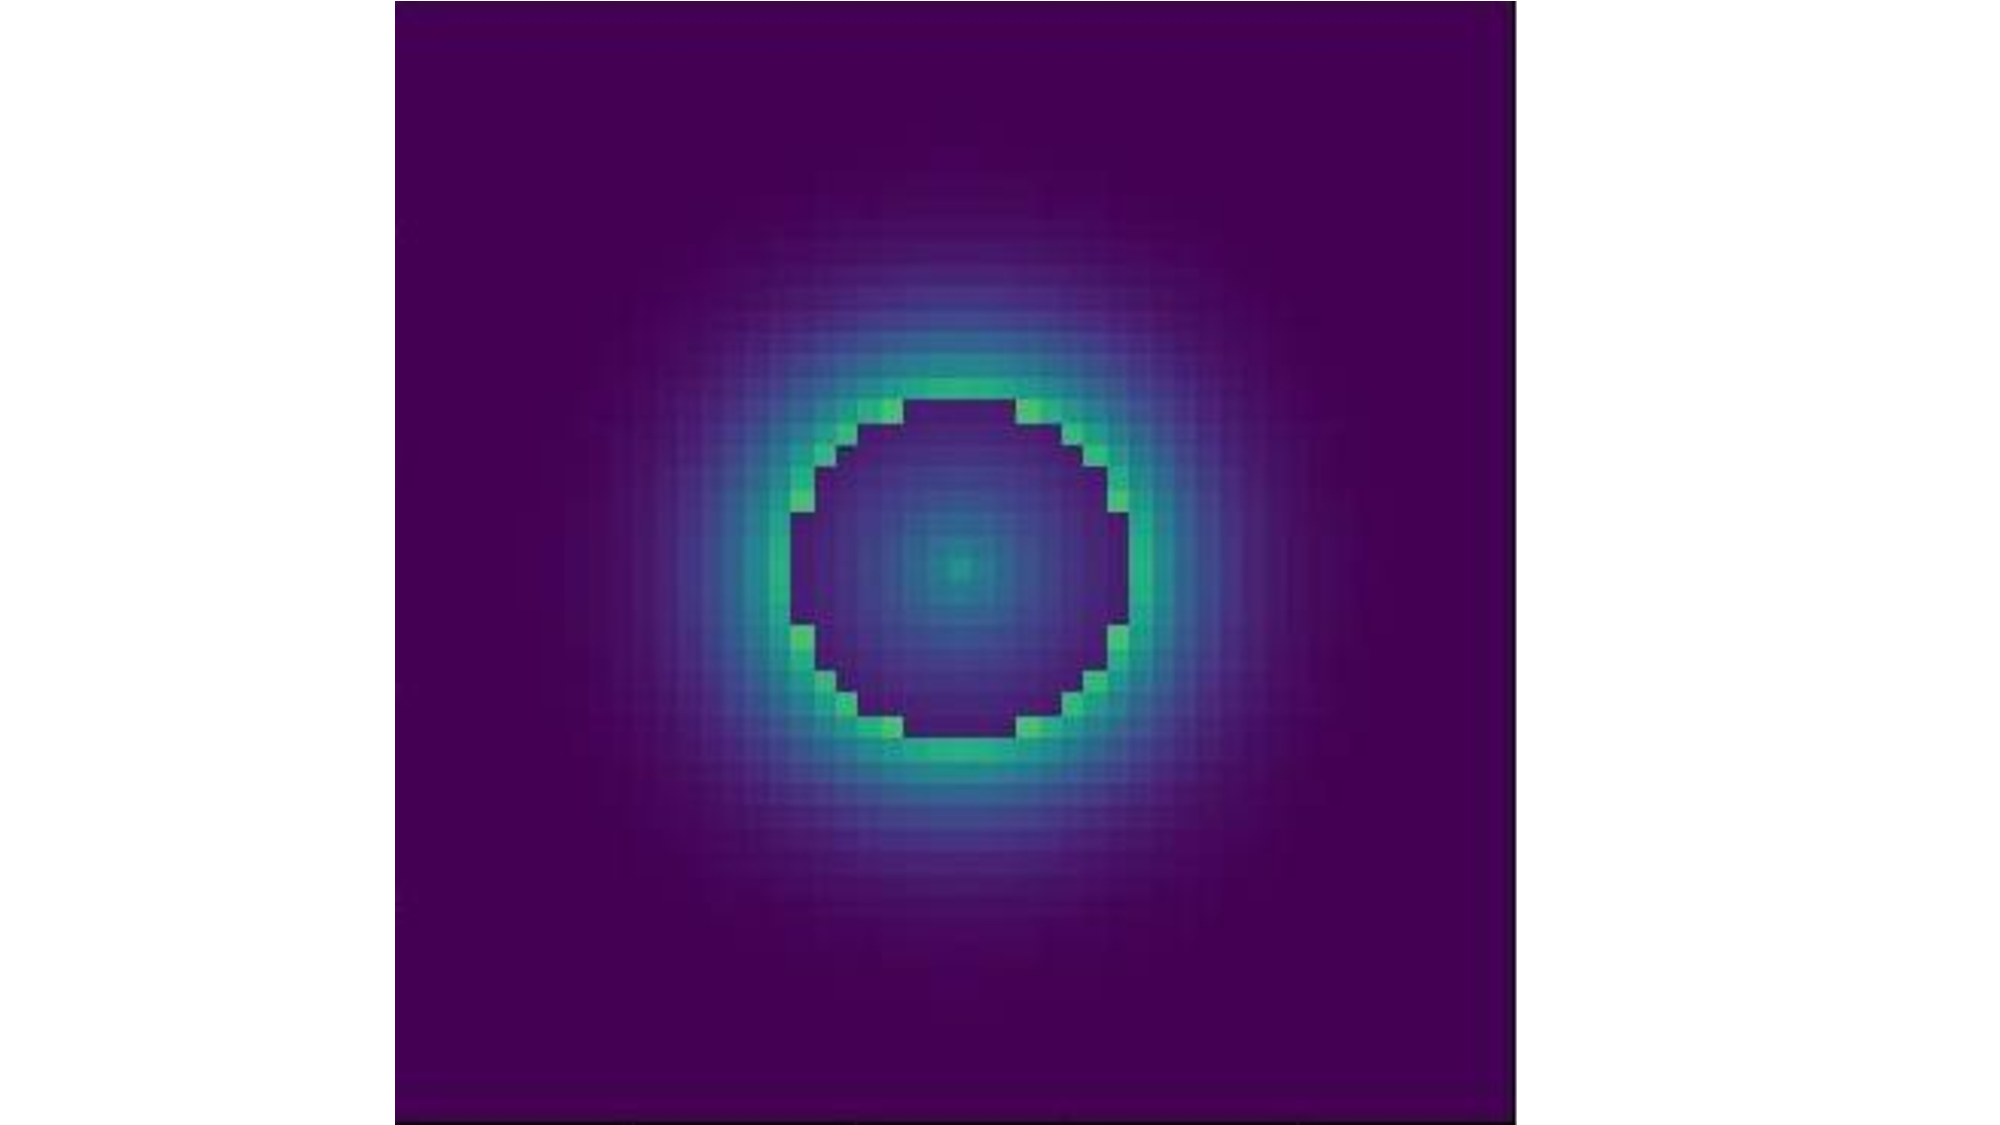
\includegraphics[width=\textwidth]{figures/raw_data/21/channel_4.pdf}
            \caption{Channel 4}
        \end{subfigure}\\
        \begin{subfigure}{0.23\textwidth}
            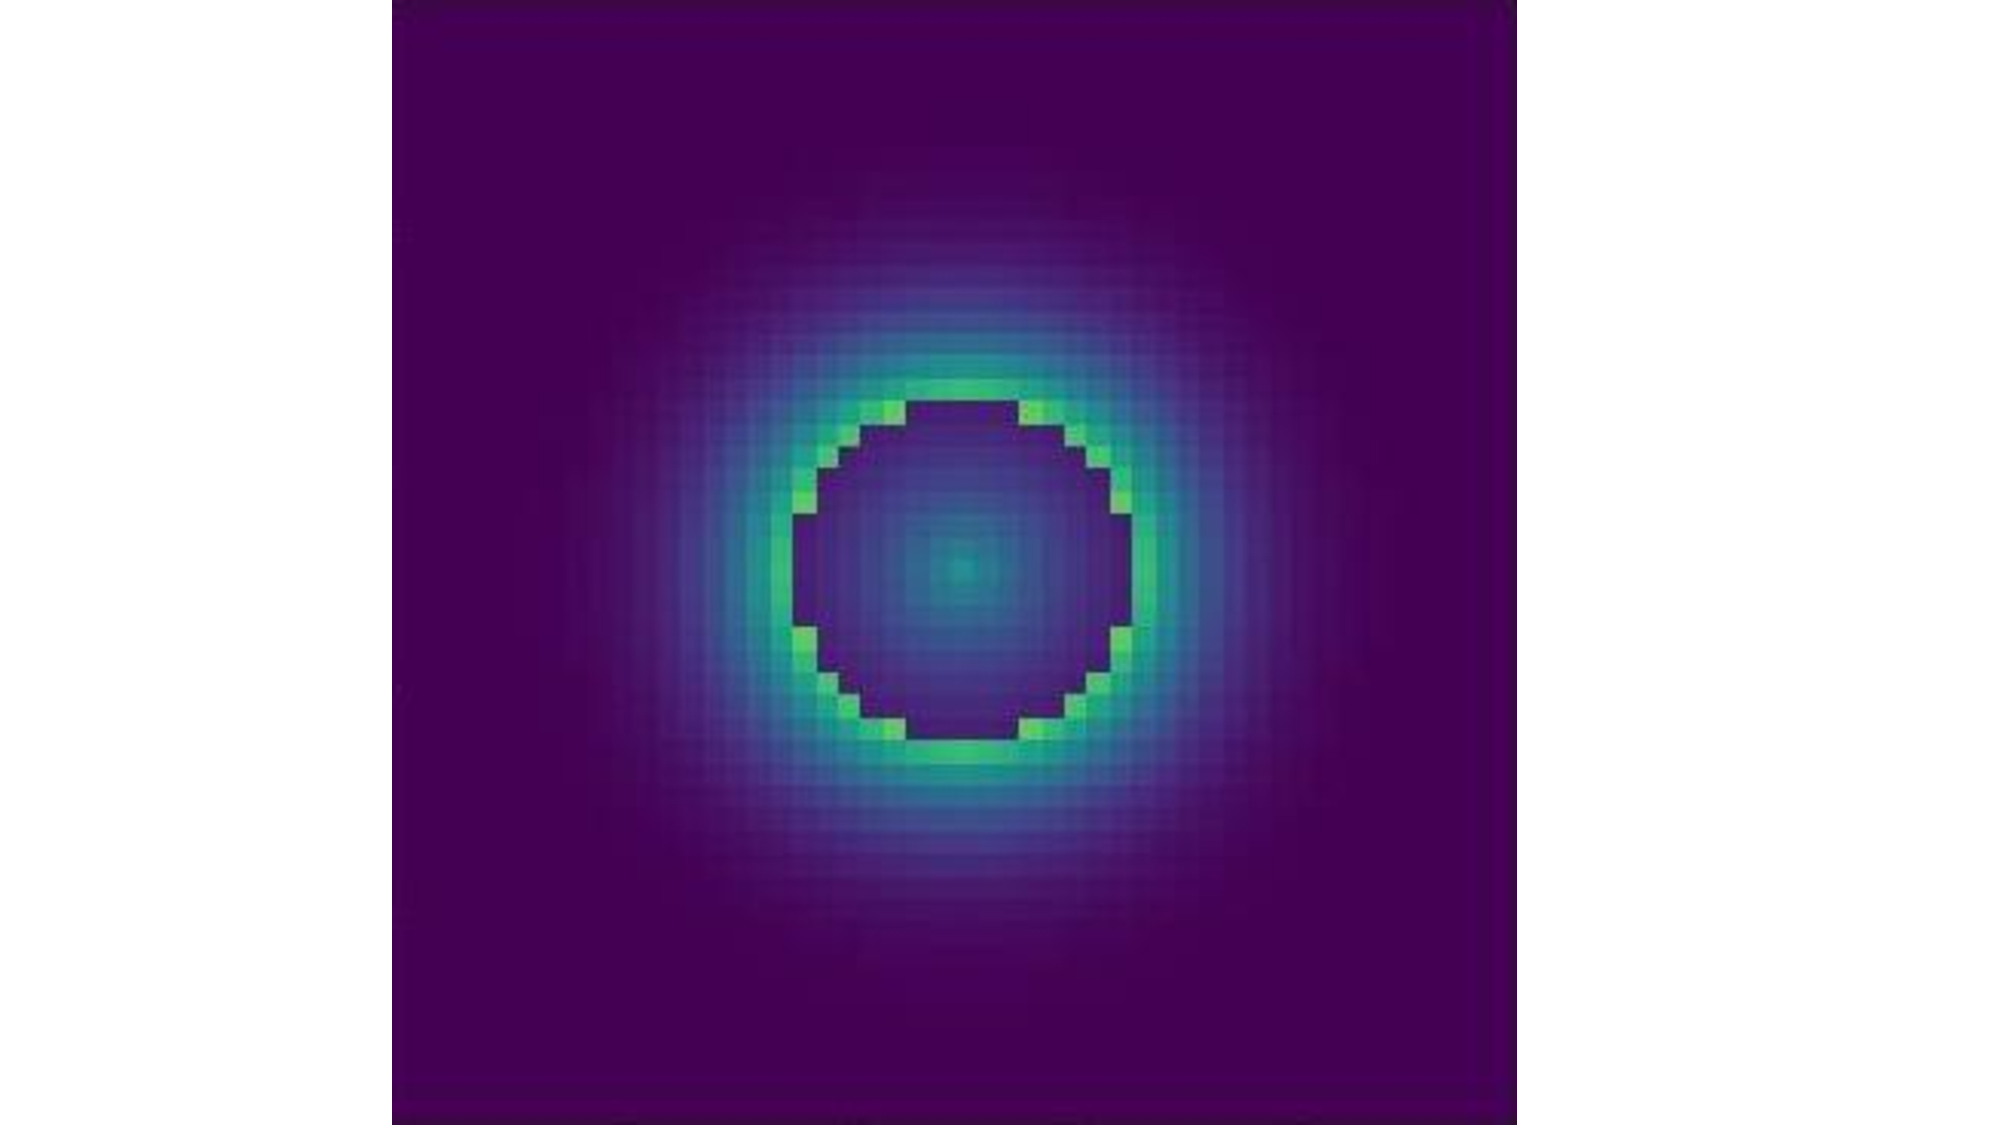
\includegraphics[width=\textwidth]{figures/raw_data/21/channel_5.pdf}
            \caption{Channel 5}
        \end{subfigure}
        \begin{subfigure}{0.23\textwidth}
            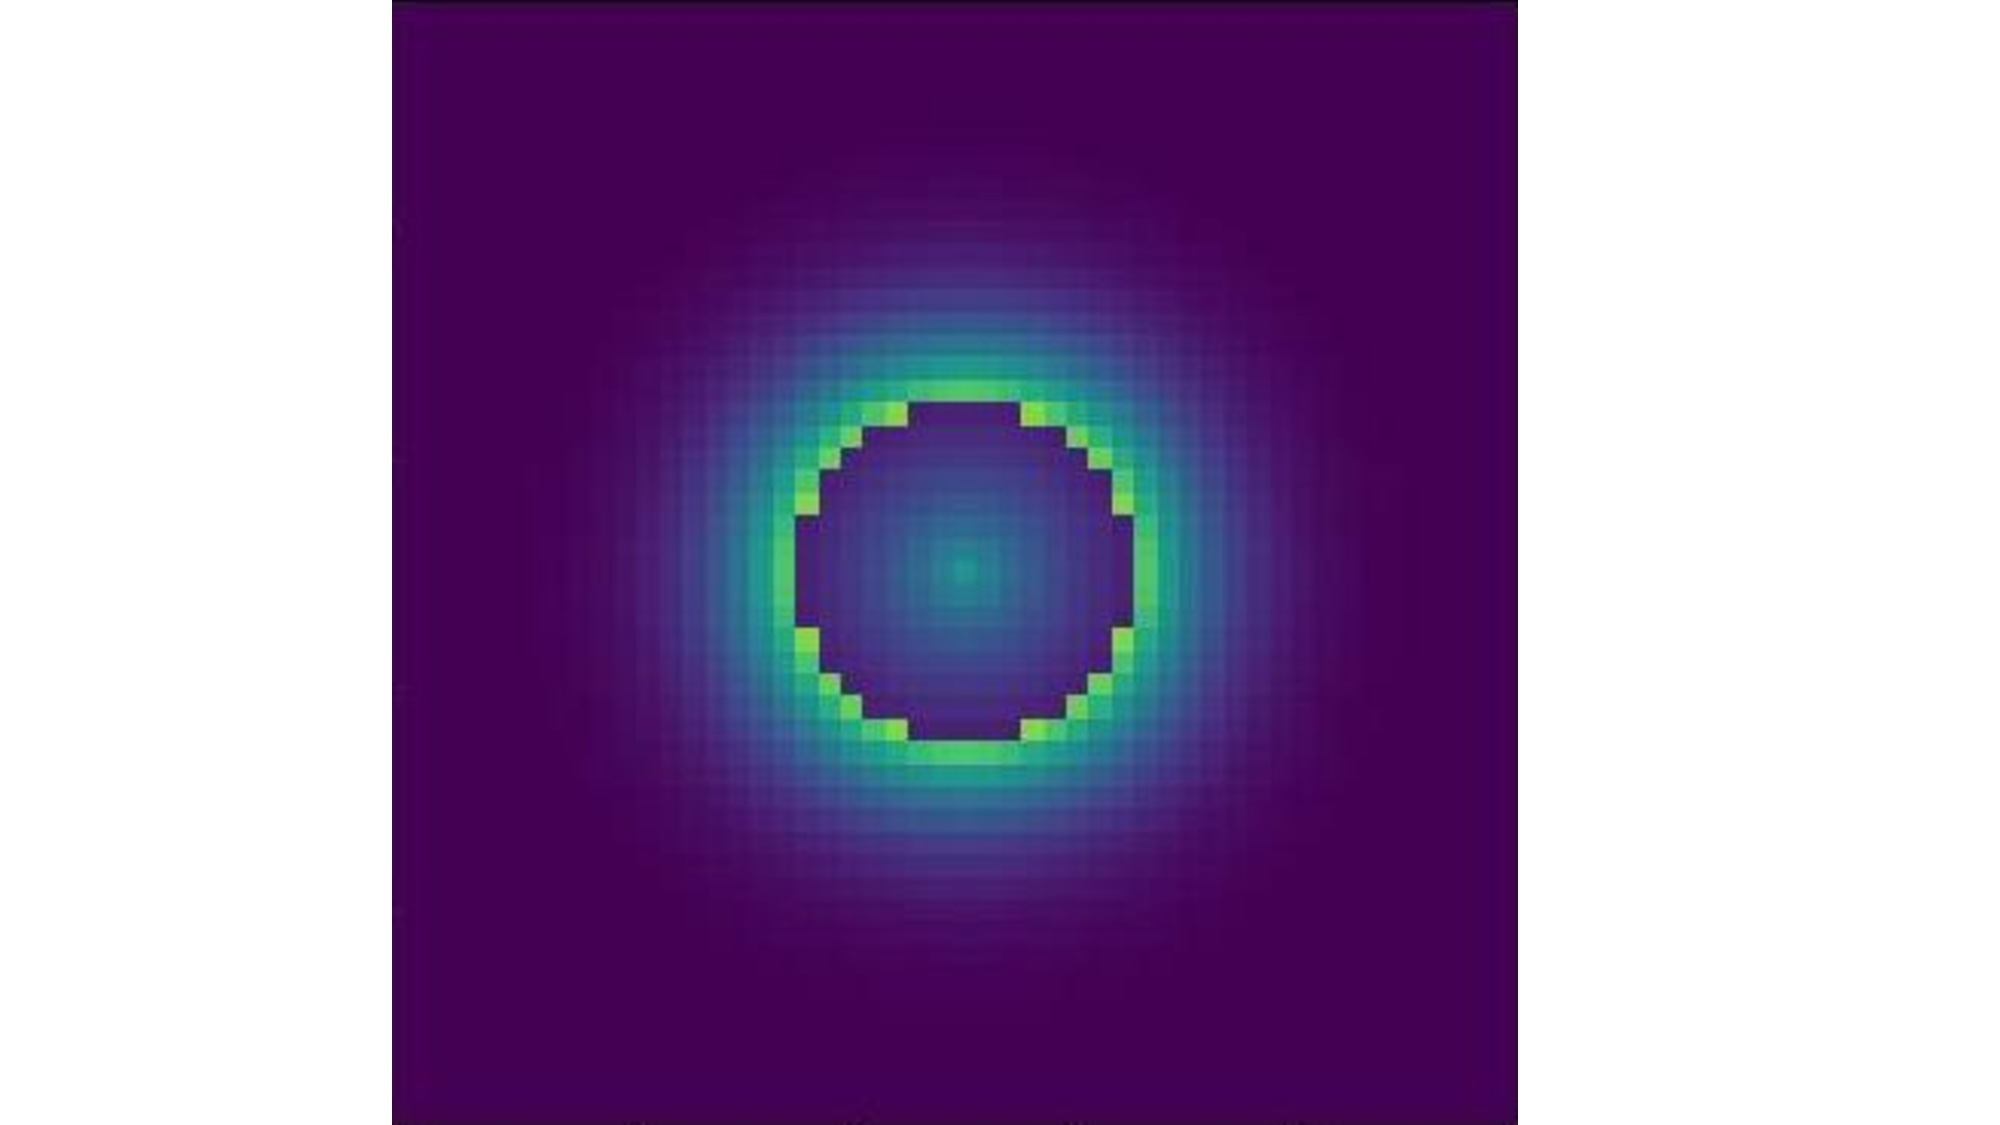
\includegraphics[width=\textwidth]{figures/raw_data/21/channel_6.pdf}
            \caption{Channel 6}
        \end{subfigure}
        \begin{subfigure}{0.23\textwidth}
            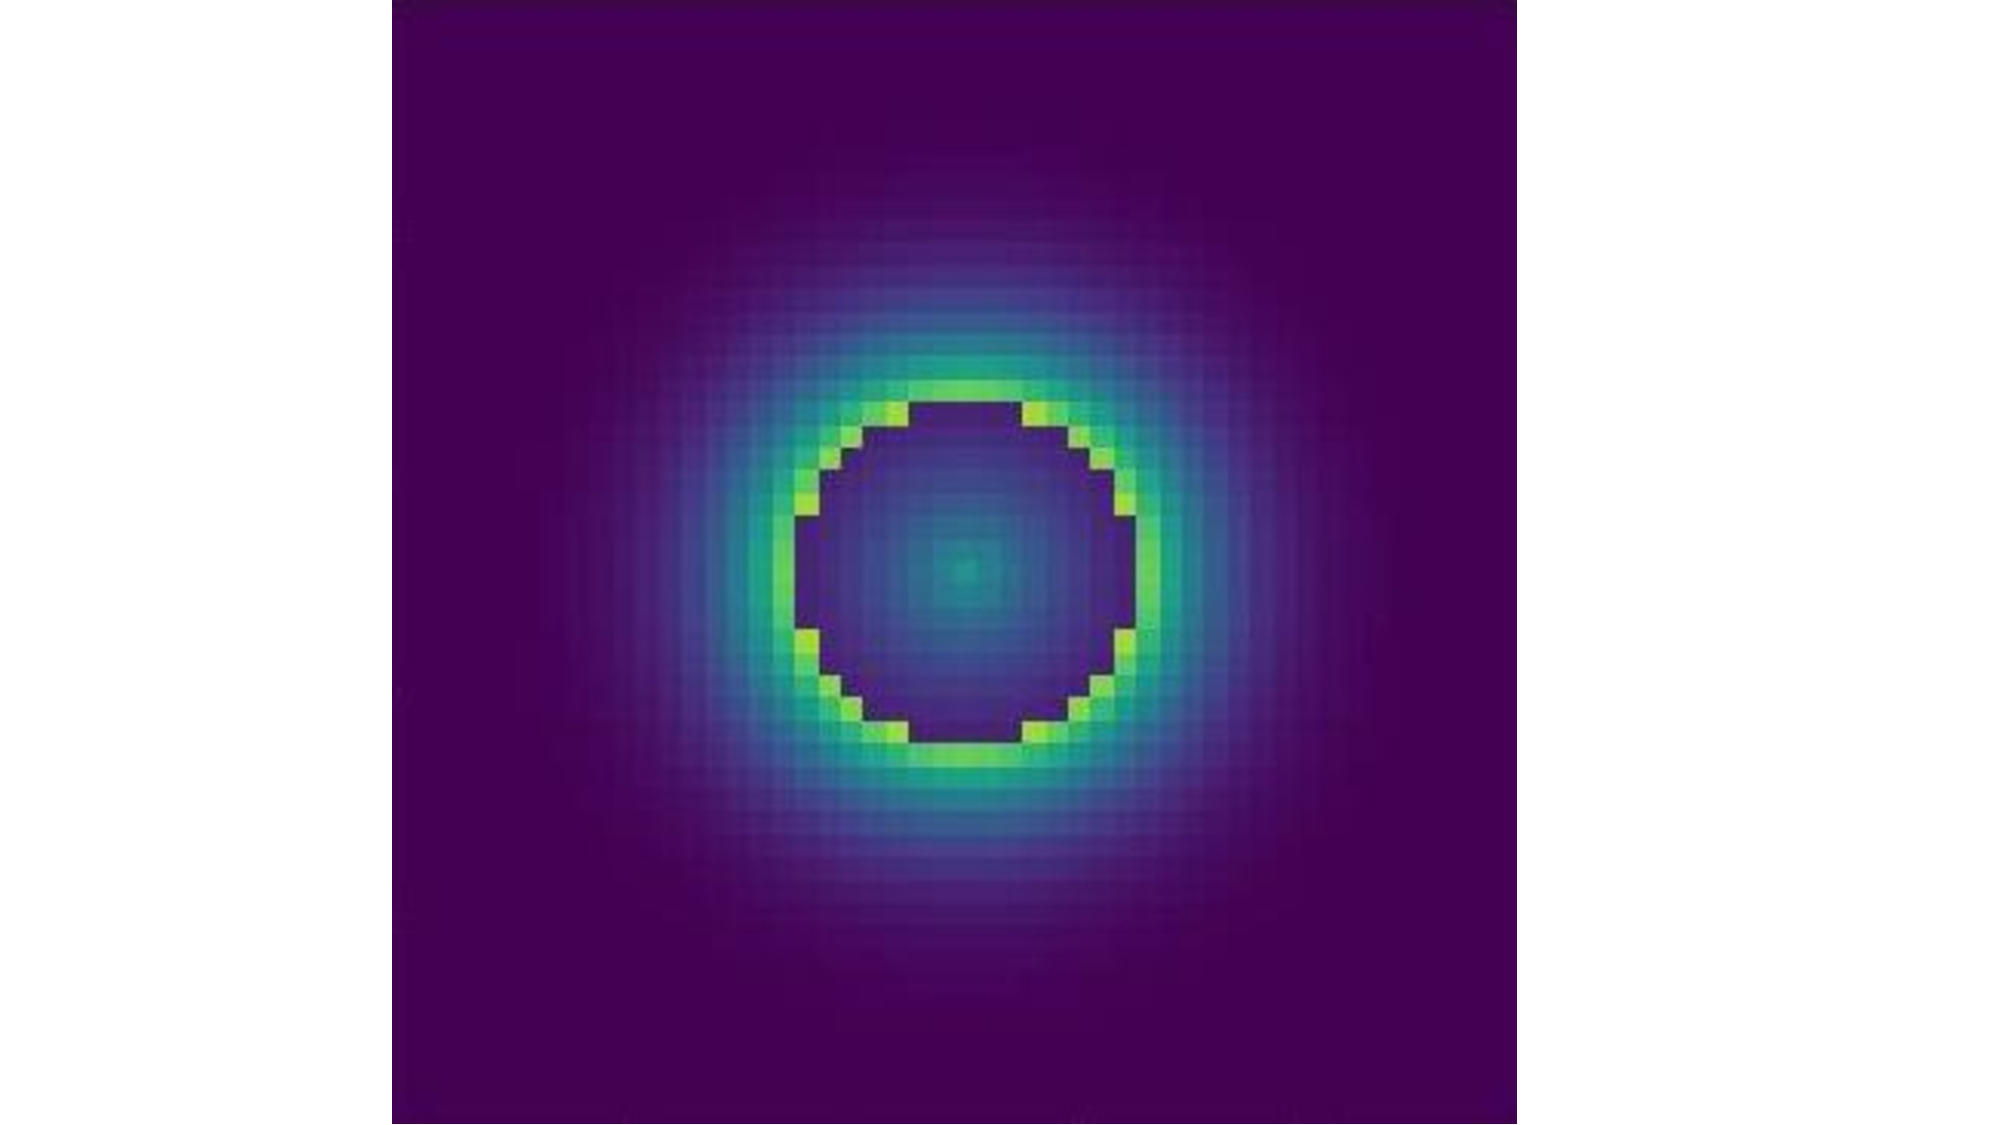
\includegraphics[width=\textwidth]{figures/raw_data/21/channel_7.pdf}
            \caption{Channel 7}
        \end{subfigure}
        \begin{subfigure}{0.23\textwidth}
            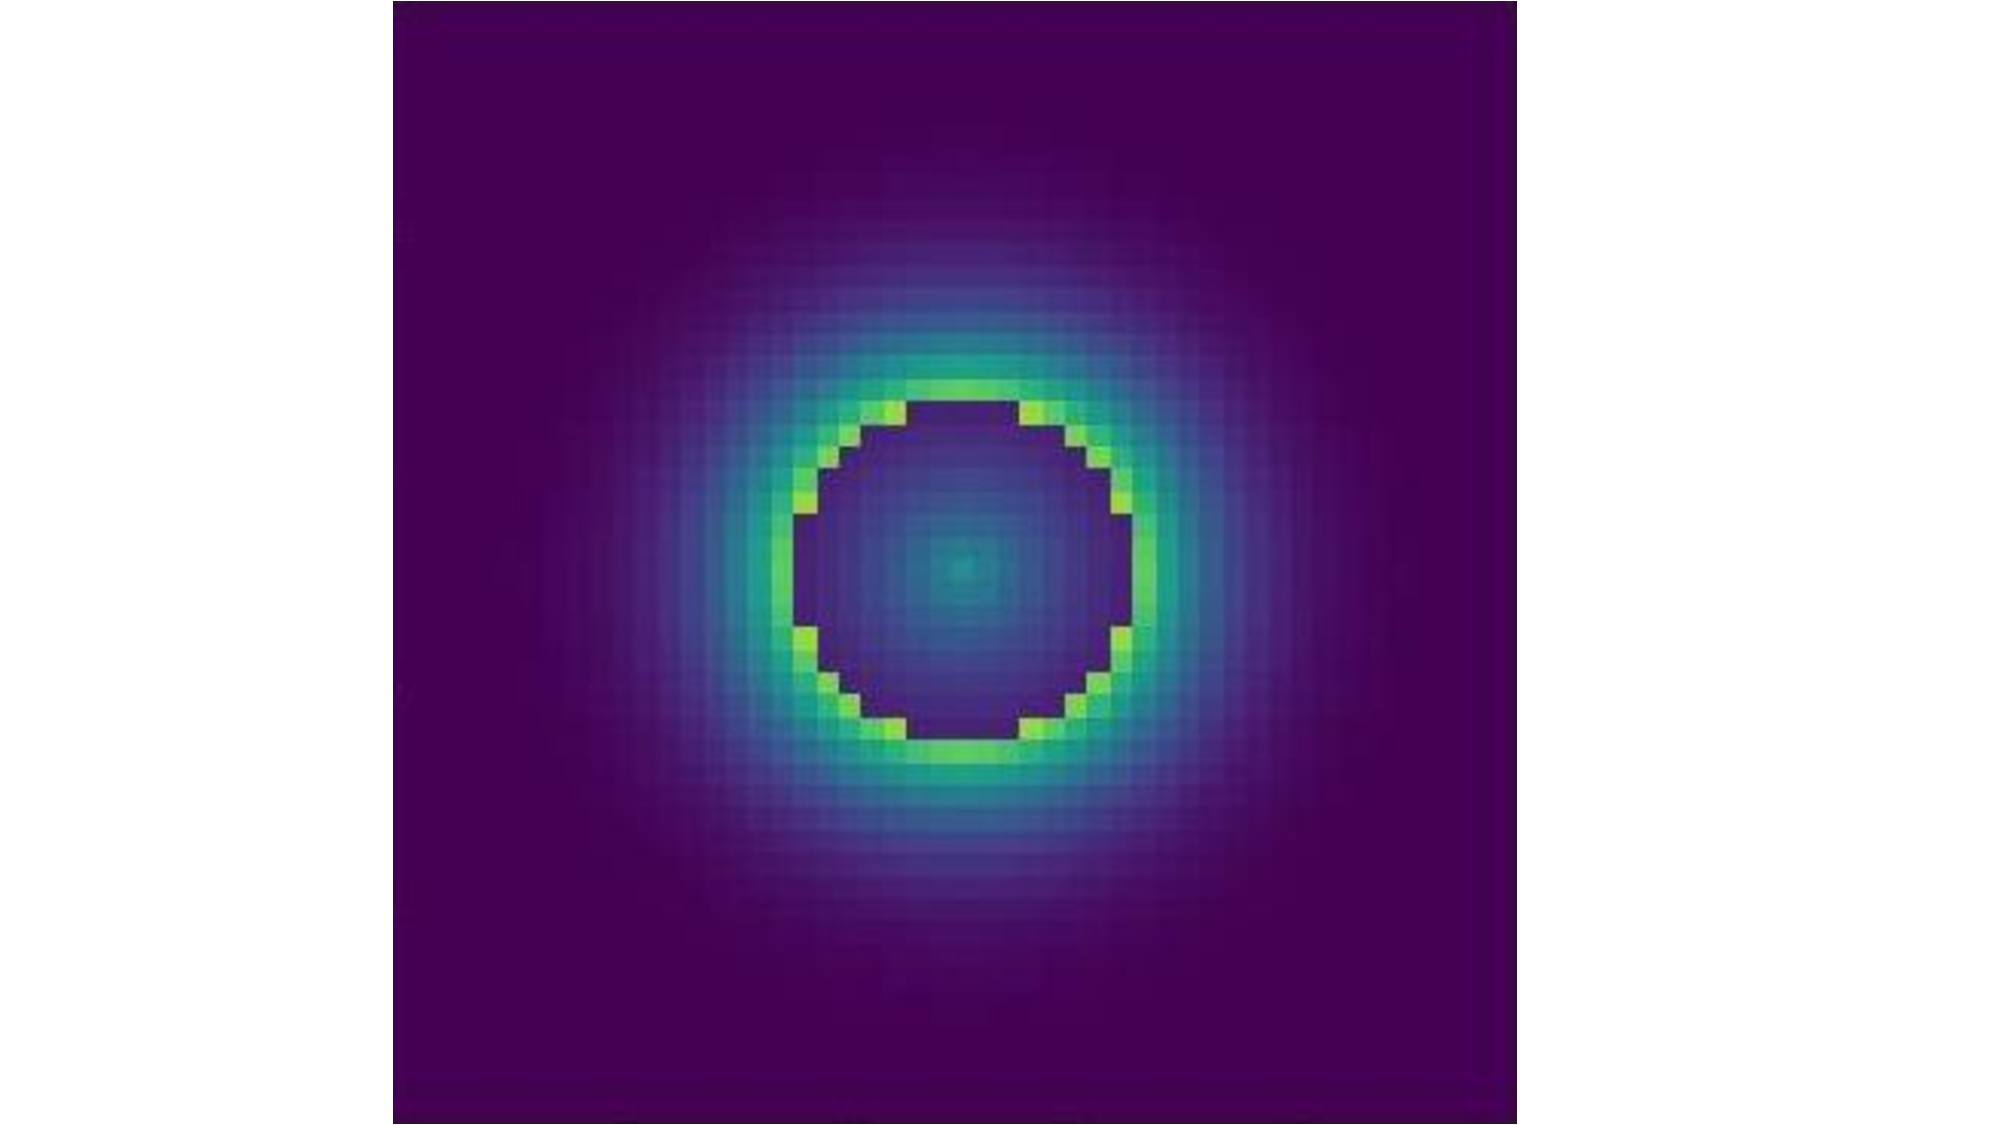
\includegraphics[width=\textwidth]{figures/raw_data/21/channel_8.pdf}
            \caption{Channel 8}
        \end{subfigure}
    \end{minipage}
    \caption{Digital value of each channel by hypothetical material based on model 1
    and a linear temperature distribution with center temperature 1900K}
    \label{fig: channel}
\end{figure}

\subsection{Estimated temperature field}
calculated temperature field
\subsection{Estimated emissivity field}
calculated emissivity field
\section{Data analysis}
use statistical method to analyse the calculated result
\subsection{Sensitivity analysis of emissivity models}
how different emissivity model affect the performance 
\subsection{Performance between different materials}
how is the performance between different materials.